% Inbuilt themes in beamer
\documentclass[aspectratio=169]{beamer}
\usepackage{graphicx}
% Theme choice:
\usetheme{CambridgeUS}

% Title page details: 
\title{Chapter 5: Elasticity and applications} 
\author{Discussion section 4}
\date{Feb 2024}

\begin{document}

% Title page
\begin{frame}
    \titlepage 
\end{frame}

% Outline frame
\begin{frame}{Outline}
    Elasticity captures an extremely intuitive concept: 
    
    \begin{center}
        How do you change your behavior in response to changing prices?
    \end{center}

    \medskip

    Let's refresh:

    \begin{center}
        When does a consumer buy more of a good?
    \end{center}

\end{frame}

\begin{frame}{Elasticity}
    \begin{enumerate}
        \item Its price is lower (law of demand)
        \item Incomes are higher (for normal goods)
        \item Price of substitutes is higher
        \item Price of complements is lower
    \end{enumerate}

    \medskip

    The \textit{elasticities of demand} will tell us just how big the change in demand is for these cases.
\end{frame}

\begin{frame}{Elasticity of demand}
    A good may have \textit{elastic} or \textit{inelastic} demand: demand responds a lot, or demand responds a little, in response to a price change.

    \medskip

    What are some examples of inelastic goods? 
    
    \medskip

    Elastic goods?

    \medskip

    \medskip

    Let's take a specific example: the Ford F-150. What factors will influence this product's elasticity of demand?
\end{frame}

\begin{frame}{Elasticity of demand}
    What factors will influence a good's elasticity?

    \begin{enumerate}
        \item \textbf{Availability of close substitutes}: other kinds of trucks, cars, bikes, etc.
        \item \textbf{Necessities vs. luxuries}: do you need it for work? For fun?
        \item \textbf{Market definition}: Are we considering the market for Ford F150s? For pickup trucks? For motor vehicles?)
        \item \textbf{Time horizon}: In the short run, maybe we need a pickup; in the long-run, maybe we retool our lives to accomadate a different car or no car at all
    \end{enumerate}
\end{frame}

\begin{frame}{Elasticity of demand}
    We have a simple equation to find the price elasticity of demand:

    $$
    \text{Price elasticity of demand} = \dfrac{\text{\% change in quantity demanded}}{\text{\% change in price}}
    $$

    Will this value be greater or less than 0? Why?

    \medskip

    First, let's refresh the basics. If good A used to cost \$10, and now it costs \$14, what is the percentage change?
\end{frame}

\begin{frame}{Elasticity of demand}
    If good A used to cost \$10, and now it costs \$14, what is the percentage change?

    $$
    \dfrac{\text{Change in price}}{\text{Original price}} * 100\% = \dfrac{\$14 - \$10}{\$10} * 100\% = 40\%
    $$

    In our elasticity formula, we do not need to worry about multiplying by 100\%.
\end{frame}

\begin{frame}{Calculating elasticity}
    Consider two points on a demand curve:
    \begin{itemize}
        \item Point A: price is $P_A=12$ and quantity demanded is $Q_A=60$
        \item Point B: $P_B=8$ and $Q_B=80$
    \end{itemize}
    Take our formula and calculate the price elasticity of demand:
    \begin{enumerate}
        \item Moving from point A to point B
        \item Moving from point B to point A
    \end{enumerate}
\end{frame}

\begin{frame}{Calculating elasticity}
    
    \begin{enumerate}
    \item Moving from point A to point B: $P_e = \dfrac{1/3}{-1/3} = -1$
    \item Moving from point B to point A: $P_e = \dfrac{-1/4}{1/2} = -\dfrac{1}{2}$
    \end{enumerate}

    Two different values! What gives?

    \medskip

    You have \$100, and lose 10\%. Tomorrow, you gain back 10\%. How much do you have?

    \medskip

    What can we do about this?

\end{frame}

\begin{frame}{Midpoint technique}
Instead of taking the \% change w.r.t. the original price, use an average of the two prices as your base,  use an average of the two:

$$
\text{Price elasticity of demand} = \dfrac{(Q_2 - Q_1)/[(Q_2 + Q_1)/2]}{(P_2 - P_1)/[(P_2 + P_1)/2]}
$$

This is the formula we will use!

\end{frame}

\begin{frame}{Calculating elasticity}
    Let's return to our example:
    \begin{itemize}
        \item $P_A=12$ and $Q_A=60$
        \item $P_B=8$ and $Q_B=80$
    \end{itemize}
    
    \medskip

    \begin{enumerate}
        \item What is the new base price?
        \item What is the new base quantity?
        \item What is the \% change for quantity?
        \item What is the \% change for price?
    \end{enumerate}

    Then put it all together to get our new elasticity estimate.
\end{frame}

\begin{frame}{Calculating elasticity}
    \begin{itemize}
        \item $P_A=12$ and $Q_A=60$
        \item $P_B=8$ and $Q_B=80$
    \end{itemize}
    
    \begin{enumerate}
        \item What is the new base price? $\$10$
        \item What is the new base quantity? $70$
        \item What is the change for quantity? $\frac{2}{7}$
        \item What is the change for price? $\frac{2}{5}$
    \end{enumerate}
\end{frame}

\begin{frame}{Calculating elasticity}
   Whether we consider moving from A to B or from B to A, we get $P_e = \dfrac{2/7}{2/5} = \dfrac{5}{7}$.

   \medskip

   Demand might be:
   \begin{itemize}
    \item Elastic
    \item Inelastic
    \item Unit elastic
    \item Perfectly elastic
    \item Perfectly inelastic
   \end{itemize}

   Group activity: draw a demand curve for each of these cases
\end{frame}

\begin{frame}{Types of elasticity}
    Demand might be:
    \begin{itemize}
     \item Elastic: price change of $X\%$ $\to$ demand change greater than $X\%$ 
     \item Inelastic: price change of $X\%$ $\to$ demand change less than $X\%$ 
     \item Unit elastic: price change of $X\%$ $\to$ demand change of $X\%$
     \item Perfectly elastic: price change has no impact on demand
     \item Perfectly inelastic: small price change has enormous impact on demand
    \end{itemize}
 \end{frame}

 \begin{frame}{Total revenue}
    How do we know how much is spent on a good at the market equilibrium?

    \medskip

    Total revenue = equilibrium price $\times$ equilibrium quantity

    \medskip

    How does elasticity interact with revenue? Think about how revenue changes when the price doubles from $P_A$ to $P_B = 2*P_A$ when:
    \begin{itemize}
        \item Demand is elastic: quantity decreases by 75\%
        \item Demand is inelastic: quantity decreases by 25\%
        \item Demand is unit elastic
    \end{itemize}

 \end{frame}

 \begin{frame}{Elasticity}
    Say we have a linear demand curve:
    \begin{itemize}
        \item Quantity demanded is 0 when price is 100
        \item Quantity demanded is 12 when price is 4
    \end{itemize}
    
    \medskip

    \begin{enumerate}
        \item Calculate the formula for the demand curve (slope and intercept) and draw graphically
        \item Is the elasticity constant? Why or why not?
        \item Pick a few example points, and use the midpoint formula to check the elasticity when:
            \begin{enumerate}
                \item Price is close to 100
                \item Price is close to 0
                \item Price is around 50
            \end{enumerate}
        \item How will total revenue vary as price moves from 0 to 100?
    \end{enumerate}

 \end{frame}

 \begin{frame}{Different elasticities}
    We have focused on the \textit{price elasticity of demand}, but there are others.

    \medskip

    In general, we can find the \textit{X elasticity of Y} as:

    $$
    \text{X elasticity of Y} = \dfrac{\%~\Delta~\text{of Y}}{\%~\Delta~\text{of X}}
    $$

    Some important elasticities:
    \begin{itemize}
        \item Income elasticity of demand
        \item Cross-price elasticity of demand
    \end{itemize}
 \end{frame}

 \begin{frame}{Different elasticities}
    Income elasticity of demand:
    \begin{itemize}
        \item Positive for normal goods, negative for inferior goods
        \item $\text{income elasticity of demand} = \dfrac{\%~\Delta~\text{of demand}}{\%~\Delta~\text{of income}}$
    \end{itemize}

    \medskip

    Cross-price elasticity of demand:
    \begin{itemize}
        \item Positive for substitutes, negative for complements
        \item $\text{CP elasticity of demand} = \dfrac{\%~\Delta~\text{of demand for good 1}}{\%~\Delta~\text{of price of good 2}}$
    \end{itemize}
 \end{frame}

 \begin{frame}{Supply elasticities}
    Firms will react to a change in price based on their \textit{price elasticity of supply}.

    \vspace{5mm}

    The same ideas are in play. Firms may have supply that is:
    \begin{itemize}
        \item elastic
        \item inelastic
        \item unit elastic
        \item perfectly elastic
        \item perfectly inelastic
    \end{itemize}

    Let's draw a graph for each of these scenarios.

    \medskip

    What is the formula for finding the price elasticity of supply?
 \end{frame}

 \begin{frame}{Supply elasticities}
    Firms may have supply that is:
    \begin{itemize}
        \item elastic: an X\% change in price $\to$ $<X\%$ change in supply
        \item inelastic: an X\% change in price $\to$ $>X\%$ change in supply
        \item unit elastic: an X\% change in price $\to$ $X\%$ change in supply
        \item perfectly elastic: any change in price $\to$ enormous change in supply
        \item perfectly inelastic: any change in price $\to$ no change in supply (perfectly vertical)
    \end{itemize}

    Of course our formula is:

    $$
    \text{price elasticity of supply} = \dfrac{\%~\Delta~\text{of supply}}{\%~\Delta~\text{of price}}
    $$

 \end{frame}

 \begin{frame}{Elasticity examples}
    Let's use some intuition, and choose three products for which we think:
    \begin{enumerate}
        \item Demand is inelastic
        \item Demand is elastic
        \item Supply is inelastic
        \item Supply is elastic
    \end{enumerate}
 \end{frame}

 \begin{frame}{Appliction}
    Let's think about the market for hotel rooms:
    \begin{table}
    \begin{tabular}{|c|c|c|c|}
      \hline
      \textbf{Price} & \textbf{$Q_D$ (Business)} & \textbf{$Q_D$ (Vacation)} & \textbf{$Q_S$ (Firms)} \\
      \hline
      \$150 & 2,100 & 1,000 & 2,300 \\
      \hline
      \$200 & 2,000 & 800   & 2,400 \\
      \hline
      \$250 & 1,900 & 600   & 2,500 \\
      \hline
      \$300 & 1,800 & 400   & 2,600 \\
      \hline
    \end{tabular}
    \caption{Market for airline tickets}
  \end{table}
    Which group do you expect to be elastic? Inelastic? Why?
    \medskip
    Calculate the elasticities.
 \end{frame}

 \begin{frame}{Appliction}
    \begin{table}
    \begin{tabular}{|c|c|c|}
      \hline
      \textbf{Business people} & \textbf{Vacationers} & \textbf{Firms} \\
      \hline
      0.17 &	0.78 &	0.15 \\ 
      0.23 &	1.29 &	0.18 \\
      \hline
      0.3	& 2.2	& 0.22 \\
      \hline
    \end{tabular}
    \caption{Elasticities for airline tickets}
  \end{table}
    Was your intuition for the elasticities correct?
    \medskip
    When is this market in \textit{equilibrium}?
 \end{frame}

%  1. Cigarettes, coffins, shoes, lightbulbs...
%  2. 5-star hotels, flights to Cancun, kitchen renovations
%  3. Stadium seats, houses, beef, microchips, missiles
%  4. Gasoline, cigarettes, 2X4s

% \begin{frame}
%     \frametitle{Demand schedule and curve}
%     \centering
%     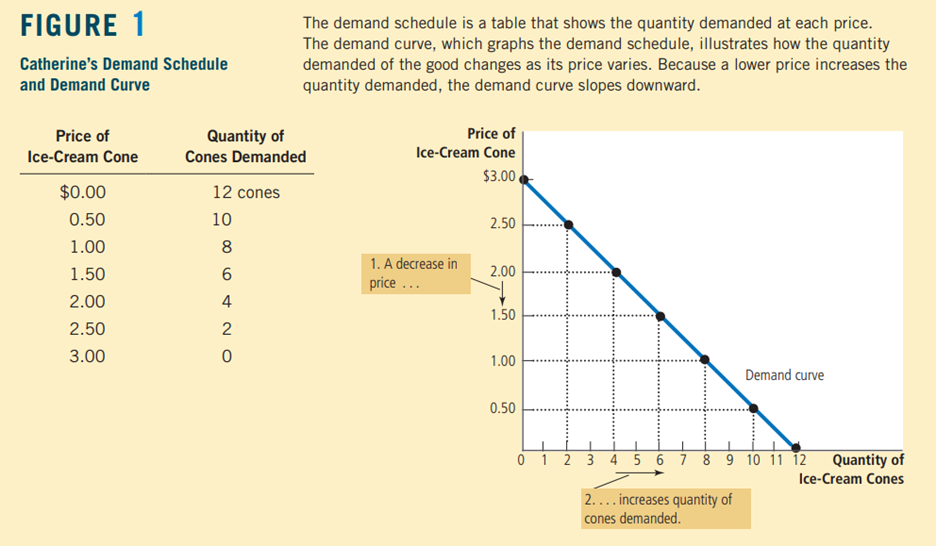
\includegraphics[width = 0.5\textwidth,keepaspectratio]{demand_curve.png}
% \end{frame}


\end{document}
